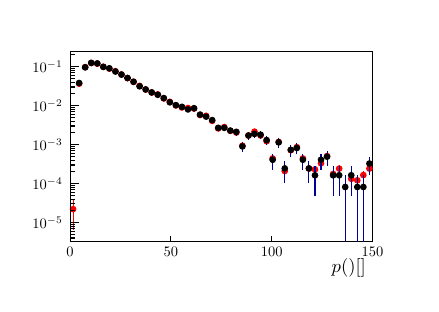
\begin{tikzpicture}
\pgfdeclareplotmark{cross} {
\pgfpathmoveto{\pgfpoint{-0.3\pgfplotmarksize}{\pgfplotmarksize}}
\pgfpathlineto{\pgfpoint{+0.3\pgfplotmarksize}{\pgfplotmarksize}}
\pgfpathlineto{\pgfpoint{+0.3\pgfplotmarksize}{0.3\pgfplotmarksize}}
\pgfpathlineto{\pgfpoint{+1\pgfplotmarksize}{0.3\pgfplotmarksize}}
\pgfpathlineto{\pgfpoint{+1\pgfplotmarksize}{-0.3\pgfplotmarksize}}
\pgfpathlineto{\pgfpoint{+0.3\pgfplotmarksize}{-0.3\pgfplotmarksize}}
\pgfpathlineto{\pgfpoint{+0.3\pgfplotmarksize}{-1.\pgfplotmarksize}}
\pgfpathlineto{\pgfpoint{-0.3\pgfplotmarksize}{-1.\pgfplotmarksize}}
\pgfpathlineto{\pgfpoint{-0.3\pgfplotmarksize}{-0.3\pgfplotmarksize}}
\pgfpathlineto{\pgfpoint{-1.\pgfplotmarksize}{-0.3\pgfplotmarksize}}
\pgfpathlineto{\pgfpoint{-1.\pgfplotmarksize}{0.3\pgfplotmarksize}}
\pgfpathlineto{\pgfpoint{-0.3\pgfplotmarksize}{0.3\pgfplotmarksize}}
\pgfpathclose
\pgfusepathqstroke
}
\pgfdeclareplotmark{cross*} {
\pgfpathmoveto{\pgfpoint{-0.3\pgfplotmarksize}{\pgfplotmarksize}}
\pgfpathlineto{\pgfpoint{+0.3\pgfplotmarksize}{\pgfplotmarksize}}
\pgfpathlineto{\pgfpoint{+0.3\pgfplotmarksize}{0.3\pgfplotmarksize}}
\pgfpathlineto{\pgfpoint{+1\pgfplotmarksize}{0.3\pgfplotmarksize}}
\pgfpathlineto{\pgfpoint{+1\pgfplotmarksize}{-0.3\pgfplotmarksize}}
\pgfpathlineto{\pgfpoint{+0.3\pgfplotmarksize}{-0.3\pgfplotmarksize}}
\pgfpathlineto{\pgfpoint{+0.3\pgfplotmarksize}{-1.\pgfplotmarksize}}
\pgfpathlineto{\pgfpoint{-0.3\pgfplotmarksize}{-1.\pgfplotmarksize}}
\pgfpathlineto{\pgfpoint{-0.3\pgfplotmarksize}{-0.3\pgfplotmarksize}}
\pgfpathlineto{\pgfpoint{-1.\pgfplotmarksize}{-0.3\pgfplotmarksize}}
\pgfpathlineto{\pgfpoint{-1.\pgfplotmarksize}{0.3\pgfplotmarksize}}
\pgfpathlineto{\pgfpoint{-0.3\pgfplotmarksize}{0.3\pgfplotmarksize}}
\pgfpathclose
\pgfusepathqfillstroke
}
\pgfdeclareplotmark{newstar} {
\pgfpathmoveto{\pgfqpoint{0pt}{\pgfplotmarksize}}
\pgfpathlineto{\pgfqpointpolar{44}{0.5\pgfplotmarksize}}
\pgfpathlineto{\pgfqpointpolar{18}{\pgfplotmarksize}}
\pgfpathlineto{\pgfqpointpolar{-20}{0.5\pgfplotmarksize}}
\pgfpathlineto{\pgfqpointpolar{-54}{\pgfplotmarksize}}
\pgfpathlineto{\pgfqpointpolar{-90}{0.5\pgfplotmarksize}}
\pgfpathlineto{\pgfqpointpolar{234}{\pgfplotmarksize}}
\pgfpathlineto{\pgfqpointpolar{198}{0.5\pgfplotmarksize}}
\pgfpathlineto{\pgfqpointpolar{162}{\pgfplotmarksize}}
\pgfpathlineto{\pgfqpointpolar{134}{0.5\pgfplotmarksize}}
\pgfpathclose
\pgfusepathqstroke
}
\pgfdeclareplotmark{newstar*} {
\pgfpathmoveto{\pgfqpoint{0pt}{\pgfplotmarksize}}
\pgfpathlineto{\pgfqpointpolar{44}{0.5\pgfplotmarksize}}
\pgfpathlineto{\pgfqpointpolar{18}{\pgfplotmarksize}}
\pgfpathlineto{\pgfqpointpolar{-20}{0.5\pgfplotmarksize}}
\pgfpathlineto{\pgfqpointpolar{-54}{\pgfplotmarksize}}
\pgfpathlineto{\pgfqpointpolar{-90}{0.5\pgfplotmarksize}}
\pgfpathlineto{\pgfqpointpolar{234}{\pgfplotmarksize}}
\pgfpathlineto{\pgfqpointpolar{198}{0.5\pgfplotmarksize}}
\pgfpathlineto{\pgfqpointpolar{162}{\pgfplotmarksize}}
\pgfpathlineto{\pgfqpointpolar{134}{0.5\pgfplotmarksize}}
\pgfpathclose
\pgfusepathqfillstroke
}
\definecolor{c}{rgb}{1,1,1};
\draw [color=c, fill=c] (5.1,0.0627517) rectangle (9.9,3.07483);
\draw [color=c, fill=c] (5.58,0.36396) rectangle (9.42,2.77362);
\definecolor{c}{rgb}{0,0,0};
\draw [c] (5.58,0.36396) -- (5.58,2.77362) -- (9.42,2.77362) -- (9.42,0.36396) -- (5.58,0.36396);
\definecolor{c}{rgb}{1,0,0};
\draw [c] (5.6184,0.512955) -- (5.6184,0.776908);
\draw [c] (5.6184,0.776908) -- (5.6184,0.891866);
\draw [c] (5.58,0.776908) -- (5.6184,0.776908);
\draw [c] (5.6184,0.776908) -- (5.6568,0.776908);
\foreach \P in {(5.6184,0.776908)}{\draw[mark options={color=c,fill=c},mark size=2.402402pt,mark=*,mark size=1pt] plot coordinates {\P};}
\draw [c] (5.6952,2.36701) -- (5.6952,2.37077);
\draw [c] (5.6952,2.37077) -- (5.6952,2.37447);
\draw [c] (5.6568,2.37077) -- (5.6952,2.37077);
\draw [c] (5.6952,2.37077) -- (5.7336,2.37077);
\foreach \P in {(5.6952,2.37077)}{\draw[mark options={color=c,fill=c},mark size=2.402402pt,mark=*,mark size=1pt] plot coordinates {\P};}
\draw [c] (5.772,2.5785) -- (5.772,2.5808);
\draw [c] (5.772,2.5808) -- (5.772,2.58308);
\draw [c] (5.7336,2.5808) -- (5.772,2.5808);
\draw [c] (5.772,2.5808) -- (5.8104,2.5808);
\foreach \P in {(5.772,2.5808)}{\draw[mark options={color=c,fill=c},mark size=2.402402pt,mark=*,mark size=1pt] plot coordinates {\P};}
\draw [c] (5.8488,2.63221) -- (5.8488,2.63424);
\draw [c] (5.8488,2.63424) -- (5.8488,2.63625);
\draw [c] (5.8104,2.63424) -- (5.8488,2.63424);
\draw [c] (5.8488,2.63424) -- (5.8872,2.63424);
\foreach \P in {(5.8488,2.63424)}{\draw[mark options={color=c,fill=c},mark size=2.402402pt,mark=*,mark size=1pt] plot coordinates {\P};}
\draw [c] (5.9256,2.62334) -- (5.9256,2.62542);
\draw [c] (5.9256,2.62542) -- (5.9256,2.62747);
\draw [c] (5.8872,2.62542) -- (5.9256,2.62542);
\draw [c] (5.9256,2.62542) -- (5.964,2.62542);
\foreach \P in {(5.9256,2.62542)}{\draw[mark options={color=c,fill=c},mark size=2.402402pt,mark=*,mark size=1pt] plot coordinates {\P};}
\draw [c] (6.0024,2.58332) -- (6.0024,2.5856);
\draw [c] (6.0024,2.5856) -- (6.0024,2.58785);
\draw [c] (5.964,2.5856) -- (6.0024,2.5856);
\draw [c] (6.0024,2.5856) -- (6.0408,2.5856);
\foreach \P in {(6.0024,2.5856)}{\draw[mark options={color=c,fill=c},mark size=2.402402pt,mark=*,mark size=1pt] plot coordinates {\P};}
\draw [c] (6.0792,2.55954) -- (6.0792,2.56195);
\draw [c] (6.0792,2.56195) -- (6.0792,2.56433);
\draw [c] (6.0408,2.56195) -- (6.0792,2.56195);
\draw [c] (6.0792,2.56195) -- (6.1176,2.56195);
\foreach \P in {(6.0792,2.56195)}{\draw[mark options={color=c,fill=c},mark size=2.402402pt,mark=*,mark size=1pt] plot coordinates {\P};}
\draw [c] (6.156,2.52583) -- (6.156,2.52843);
\draw [c] (6.156,2.52843) -- (6.156,2.531);
\draw [c] (6.1176,2.52843) -- (6.156,2.52843);
\draw [c] (6.156,2.52843) -- (6.1944,2.52843);
\foreach \P in {(6.156,2.52843)}{\draw[mark options={color=c,fill=c},mark size=2.402402pt,mark=*,mark size=1pt] plot coordinates {\P};}
\draw [c] (6.2328,2.48391) -- (6.2328,2.48678);
\draw [c] (6.2328,2.48678) -- (6.2328,2.48961);
\draw [c] (6.1944,2.48678) -- (6.2328,2.48678);
\draw [c] (6.2328,2.48678) -- (6.2712,2.48678);
\foreach \P in {(6.2328,2.48678)}{\draw[mark options={color=c,fill=c},mark size=2.402402pt,mark=*,mark size=1pt] plot coordinates {\P};}
\draw [c] (6.3096,2.43766) -- (6.3096,2.44085);
\draw [c] (6.3096,2.44085) -- (6.3096,2.44399);
\draw [c] (6.2712,2.44085) -- (6.3096,2.44085);
\draw [c] (6.3096,2.44085) -- (6.348,2.44085);
\foreach \P in {(6.3096,2.44085)}{\draw[mark options={color=c,fill=c},mark size=2.402402pt,mark=*,mark size=1pt] plot coordinates {\P};}
\draw [c] (6.3864,2.39219) -- (6.3864,2.39574);
\draw [c] (6.3864,2.39574) -- (6.3864,2.39923);
\draw [c] (6.348,2.39574) -- (6.3864,2.39574);
\draw [c] (6.3864,2.39574) -- (6.4248,2.39574);
\foreach \P in {(6.3864,2.39574)}{\draw[mark options={color=c,fill=c},mark size=2.402402pt,mark=*,mark size=1pt] plot coordinates {\P};}
\draw [c] (6.4632,2.33783) -- (6.4632,2.34186);
\draw [c] (6.4632,2.34186) -- (6.4632,2.34581);
\draw [c] (6.4248,2.34186) -- (6.4632,2.34186);
\draw [c] (6.4632,2.34186) -- (6.5016,2.34186);
\foreach \P in {(6.4632,2.34186)}{\draw[mark options={color=c,fill=c},mark size=2.402402pt,mark=*,mark size=1pt] plot coordinates {\P};}
\draw [c] (6.54,2.29241) -- (6.54,2.29689);
\draw [c] (6.54,2.29689) -- (6.54,2.30127);
\draw [c] (6.5016,2.29689) -- (6.54,2.29689);
\draw [c] (6.54,2.29689) -- (6.5784,2.29689);
\foreach \P in {(6.54,2.29689)}{\draw[mark options={color=c,fill=c},mark size=2.402402pt,mark=*,mark size=1pt] plot coordinates {\P};}
\draw [c] (6.6168,2.25384) -- (6.6168,2.25873);
\draw [c] (6.6168,2.25873) -- (6.6168,2.26352);
\draw [c] (6.5784,2.25873) -- (6.6168,2.25873);
\draw [c] (6.6168,2.25873) -- (6.6552,2.25873);
\foreach \P in {(6.6168,2.25873)}{\draw[mark options={color=c,fill=c},mark size=2.402402pt,mark=*,mark size=1pt] plot coordinates {\P};}
\draw [c] (6.6936,2.22811) -- (6.6936,2.23331);
\draw [c] (6.6936,2.23331) -- (6.6936,2.23838);
\draw [c] (6.6552,2.23331) -- (6.6936,2.23331);
\draw [c] (6.6936,2.23331) -- (6.732,2.23331);
\foreach \P in {(6.6936,2.23331)}{\draw[mark options={color=c,fill=c},mark size=2.402402pt,mark=*,mark size=1pt] plot coordinates {\P};}
\draw [c] (6.7704,2.1774) -- (6.7704,2.18324);
\draw [c] (6.7704,2.18324) -- (6.7704,2.18894);
\draw [c] (6.732,2.18324) -- (6.7704,2.18324);
\draw [c] (6.7704,2.18324) -- (6.8088,2.18324);
\foreach \P in {(6.7704,2.18324)}{\draw[mark options={color=c,fill=c},mark size=2.402402pt,mark=*,mark size=1pt] plot coordinates {\P};}
\draw [c] (6.8472,2.13313) -- (6.8472,2.13961);
\draw [c] (6.8472,2.13961) -- (6.8472,2.1459);
\draw [c] (6.8088,2.13961) -- (6.8472,2.13961);
\draw [c] (6.8472,2.13961) -- (6.8856,2.13961);
\foreach \P in {(6.8472,2.13961)}{\draw[mark options={color=c,fill=c},mark size=2.402402pt,mark=*,mark size=1pt] plot coordinates {\P};}
\draw [c] (6.924,2.08693) -- (6.924,2.09414);
\draw [c] (6.924,2.09414) -- (6.924,2.10113);
\draw [c] (6.8856,2.09414) -- (6.924,2.09414);
\draw [c] (6.924,2.09414) -- (6.9624,2.09414);
\foreach \P in {(6.924,2.09414)}{\draw[mark options={color=c,fill=c},mark size=2.402402pt,mark=*,mark size=1pt] plot coordinates {\P};}
\draw [c] (7.0008,2.0614) -- (7.0008,2.06906);
\draw [c] (7.0008,2.06906) -- (7.0008,2.07646);
\draw [c] (6.9624,2.06906) -- (7.0008,2.06906);
\draw [c] (7.0008,2.06906) -- (7.0392,2.06906);
\foreach \P in {(7.0008,2.06906)}{\draw[mark options={color=c,fill=c},mark size=2.402402pt,mark=*,mark size=1pt] plot coordinates {\P};}
\draw [c] (7.0776,2.0532) -- (7.0776,2.06101);
\draw [c] (7.0776,2.06101) -- (7.0776,2.06854);
\draw [c] (7.0392,2.06101) -- (7.0776,2.06101);
\draw [c] (7.0776,2.06101) -- (7.116,2.06101);
\foreach \P in {(7.0776,2.06101)}{\draw[mark options={color=c,fill=c},mark size=2.402402pt,mark=*,mark size=1pt] plot coordinates {\P};}
\draw [c] (7.1544,2.04641) -- (7.1544,2.05434);
\draw [c] (7.1544,2.05434) -- (7.1544,2.06199);
\draw [c] (7.116,2.05434) -- (7.1544,2.05434);
\draw [c] (7.1544,2.05434) -- (7.1928,2.05434);
\foreach \P in {(7.1544,2.05434)}{\draw[mark options={color=c,fill=c},mark size=2.402402pt,mark=*,mark size=1pt] plot coordinates {\P};}
\draw [c] (7.2312,1.96256) -- (7.2312,1.9722);
\draw [c] (7.2312,1.9722) -- (7.2312,1.98143);
\draw [c] (7.1928,1.9722) -- (7.2312,1.9722);
\draw [c] (7.2312,1.9722) -- (7.2696,1.9722);
\foreach \P in {(7.2312,1.9722)}{\draw[mark options={color=c,fill=c},mark size=2.402402pt,mark=*,mark size=1pt] plot coordinates {\P};}
\draw [c] (7.308,1.95261) -- (7.308,1.96248);
\draw [c] (7.308,1.96248) -- (7.308,1.97191);
\draw [c] (7.2696,1.96248) -- (7.308,1.96248);
\draw [c] (7.308,1.96248) -- (7.3464,1.96248);
\foreach \P in {(7.308,1.96248)}{\draw[mark options={color=c,fill=c},mark size=2.402402pt,mark=*,mark size=1pt] plot coordinates {\P};}
\draw [c] (7.3848,1.88698) -- (7.3848,1.89847);
\draw [c] (7.3848,1.89847) -- (7.3848,1.90938);
\draw [c] (7.3464,1.89847) -- (7.3848,1.89847);
\draw [c] (7.3848,1.89847) -- (7.4232,1.89847);
\foreach \P in {(7.3848,1.89847)}{\draw[mark options={color=c,fill=c},mark size=2.402402pt,mark=*,mark size=1pt] plot coordinates {\P};}
\draw [c] (7.4616,1.78792) -- (7.4616,1.80239);
\draw [c] (7.4616,1.80239) -- (7.4616,1.81595);
\draw [c] (7.4232,1.80239) -- (7.4616,1.80239);
\draw [c] (7.4616,1.80239) -- (7.5,1.80239);
\foreach \P in {(7.4616,1.80239)}{\draw[mark options={color=c,fill=c},mark size=2.402402pt,mark=*,mark size=1pt] plot coordinates {\P};}
\draw [c] (7.5384,1.80513) -- (7.5384,1.81903);
\draw [c] (7.5384,1.81903) -- (7.5384,1.83209);
\draw [c] (7.5,1.81903) -- (7.5384,1.81903);
\draw [c] (7.5384,1.81903) -- (7.5768,1.81903);
\foreach \P in {(7.5384,1.81903)}{\draw[mark options={color=c,fill=c},mark size=2.402402pt,mark=*,mark size=1pt] plot coordinates {\P};}
\draw [c] (7.6152,1.75656) -- (7.6152,1.77212);
\draw [c] (7.6152,1.77212) -- (7.6152,1.78663);
\draw [c] (7.5768,1.77212) -- (7.6152,1.77212);
\draw [c] (7.6152,1.77212) -- (7.6536,1.77212);
\foreach \P in {(7.6152,1.77212)}{\draw[mark options={color=c,fill=c},mark size=2.402402pt,mark=*,mark size=1pt] plot coordinates {\P};}
\draw [c] (7.692,1.73364) -- (7.692,1.75005);
\draw [c] (7.692,1.75005) -- (7.692,1.7653);
\draw [c] (7.6536,1.75005) -- (7.692,1.75005);
\draw [c] (7.692,1.75005) -- (7.7304,1.75005);
\foreach \P in {(7.692,1.75005)}{\draw[mark options={color=c,fill=c},mark size=2.402402pt,mark=*,mark size=1pt] plot coordinates {\P};}
\draw [c] (7.7688,1.5582) -- (7.7688,1.58288);
\draw [c] (7.7688,1.58288) -- (7.7688,1.60502);
\draw [c] (7.7304,1.58288) -- (7.7688,1.58288);
\draw [c] (7.7688,1.58288) -- (7.8072,1.58288);
\foreach \P in {(7.7688,1.58288)}{\draw[mark options={color=c,fill=c},mark size=2.402402pt,mark=*,mark size=1pt] plot coordinates {\P};}
\draw [c] (7.8456,1.69402) -- (7.8456,1.71202);
\draw [c] (7.8456,1.71202) -- (7.8456,1.72863);
\draw [c] (7.8072,1.71202) -- (7.8456,1.71202);
\draw [c] (7.8456,1.71202) -- (7.884,1.71202);
\foreach \P in {(7.8456,1.71202)}{\draw[mark options={color=c,fill=c},mark size=2.402402pt,mark=*,mark size=1pt] plot coordinates {\P};}
\draw [c] (7.9224,1.7454) -- (7.9224,1.76137);
\draw [c] (7.9224,1.76137) -- (7.9224,1.77624);
\draw [c] (7.884,1.76137) -- (7.9224,1.76137);
\draw [c] (7.9224,1.76137) -- (7.9608,1.76137);
\foreach \P in {(7.9224,1.76137)}{\draw[mark options={color=c,fill=c},mark size=2.402402pt,mark=*,mark size=1pt] plot coordinates {\P};}
\draw [c] (7.9992,1.69547) -- (7.9992,1.7134);
\draw [c] (7.9992,1.7134) -- (7.9992,1.72996);
\draw [c] (7.9608,1.7134) -- (7.9992,1.7134);
\draw [c] (7.9992,1.7134) -- (8.0376,1.7134);
\foreach \P in {(7.9992,1.7134)}{\draw[mark options={color=c,fill=c},mark size=2.402402pt,mark=*,mark size=1pt] plot coordinates {\P};}
\draw [c] (8.076,1.61881) -- (8.076,1.64025);
\draw [c] (8.076,1.64025) -- (8.076,1.65974);
\draw [c] (8.0376,1.64025) -- (8.076,1.64025);
\draw [c] (8.076,1.64025) -- (8.1144,1.64025);
\foreach \P in {(8.076,1.64025)}{\draw[mark options={color=c,fill=c},mark size=2.402402pt,mark=*,mark size=1pt] plot coordinates {\P};}
\draw [c] (8.1528,1.38386) -- (8.1528,1.42086);
\draw [c] (8.1528,1.42086) -- (8.1528,1.45241);
\draw [c] (8.1144,1.42086) -- (8.1528,1.42086);
\draw [c] (8.1528,1.42086) -- (8.1912,1.42086);
\foreach \P in {(8.1528,1.42086)}{\draw[mark options={color=c,fill=c},mark size=2.402402pt,mark=*,mark size=1pt] plot coordinates {\P};}
\draw [c] (8.2296,1.60838) -- (8.2296,1.63034);
\draw [c] (8.2296,1.63034) -- (8.2296,1.65027);
\draw [c] (8.1912,1.63034) -- (8.2296,1.63034);
\draw [c] (8.2296,1.63034) -- (8.268,1.63034);
\foreach \P in {(8.2296,1.63034)}{\draw[mark options={color=c,fill=c},mark size=2.402402pt,mark=*,mark size=1pt] plot coordinates {\P};}
\draw [c] (8.3064,1.20482) -- (8.3064,1.26083);
\draw [c] (8.3064,1.26083) -- (8.3064,1.30523);
\draw [c] (8.268,1.26083) -- (8.3064,1.26083);
\draw [c] (8.3064,1.26083) -- (8.3448,1.26083);
\foreach \P in {(8.3064,1.26083)}{\draw[mark options={color=c,fill=c},mark size=2.402402pt,mark=*,mark size=1pt] plot coordinates {\P};}
\draw [c] (8.3832,1.49675) -- (8.3832,1.52522);
\draw [c] (8.3832,1.52522) -- (8.3832,1.55035);
\draw [c] (8.3448,1.52522) -- (8.3832,1.52522);
\draw [c] (8.3832,1.52522) -- (8.4216,1.52522);
\foreach \P in {(8.3832,1.52522)}{\draw[mark options={color=c,fill=c},mark size=2.402402pt,mark=*,mark size=1pt] plot coordinates {\P};}
\draw [c] (8.46,1.53858) -- (8.46,1.56441);
\draw [c] (8.46,1.56441) -- (8.46,1.58747);
\draw [c] (8.4216,1.56441) -- (8.46,1.56441);
\draw [c] (8.46,1.56441) -- (8.4984,1.56441);
\foreach \P in {(8.46,1.56441)}{\draw[mark options={color=c,fill=c},mark size=2.402402pt,mark=*,mark size=1pt] plot coordinates {\P};}
\draw [c] (8.5368,1.38386) -- (8.5368,1.42086);
\draw [c] (8.5368,1.42086) -- (8.5368,1.45241);
\draw [c] (8.4984,1.42086) -- (8.5368,1.42086);
\draw [c] (8.5368,1.42086) -- (8.5752,1.42086);
\foreach \P in {(8.5368,1.42086)}{\draw[mark options={color=c,fill=c},mark size=2.402402pt,mark=*,mark size=1pt] plot coordinates {\P};}
\draw [c] (8.6136,1.24081) -- (8.6136,1.29235);
\draw [c] (8.6136,1.29235) -- (8.6136,1.33389);
\draw [c] (8.5752,1.29235) -- (8.6136,1.29235);
\draw [c] (8.6136,1.29235) -- (8.652,1.29235);
\foreach \P in {(8.6136,1.29235)}{\draw[mark options={color=c,fill=c},mark size=2.402402pt,mark=*,mark size=1pt] plot coordinates {\P};}
\draw [c] (8.6904,1.22943) -- (8.6904,1.28235);
\draw [c] (8.6904,1.28235) -- (8.6904,1.32478);
\draw [c] (8.652,1.28235) -- (8.6904,1.28235);
\draw [c] (8.6904,1.28235) -- (8.7288,1.28235);
\foreach \P in {(8.6904,1.28235)}{\draw[mark options={color=c,fill=c},mark size=2.402402pt,mark=*,mark size=1pt] plot coordinates {\P};}
\draw [c] (8.7672,1.31568) -- (8.7672,1.35902);
\draw [c] (8.7672,1.35902) -- (8.7672,1.39506);
\draw [c] (8.7288,1.35902) -- (8.7672,1.35902);
\draw [c] (8.7672,1.35902) -- (8.8056,1.35902);
\foreach \P in {(8.7672,1.35902)}{\draw[mark options={color=c,fill=c},mark size=2.402402pt,mark=*,mark size=1pt] plot coordinates {\P};}
\draw [c] (8.844,1.41661) -- (8.844,1.4509);
\draw [c] (8.844,1.4509) -- (8.844,1.48046);
\draw [c] (8.8056,1.4509) -- (8.844,1.4509);
\draw [c] (8.844,1.4509) -- (8.8824,1.4509);
\foreach \P in {(8.844,1.4509)}{\draw[mark options={color=c,fill=c},mark size=2.402402pt,mark=*,mark size=1pt] plot coordinates {\P};}
\draw [c] (8.9208,1.16206) -- (8.9208,1.22389);
\draw [c] (8.9208,1.22389) -- (8.9208,1.27186);
\draw [c] (8.8824,1.22389) -- (8.9208,1.22389);
\draw [c] (8.9208,1.22389) -- (8.9592,1.22389);
\foreach \P in {(8.9208,1.22389)}{\draw[mark options={color=c,fill=c},mark size=2.402402pt,mark=*,mark size=1pt] plot coordinates {\P};}
\draw [c] (8.9976,1.24081) -- (8.9976,1.29235);
\draw [c] (8.9976,1.29235) -- (8.9976,1.33389);
\draw [c] (8.9592,1.29235) -- (8.9976,1.29235);
\draw [c] (8.9976,1.29235) -- (9.036,1.29235);
\foreach \P in {(8.9976,1.29235)}{\draw[mark options={color=c,fill=c},mark size=2.402402pt,mark=*,mark size=1pt] plot coordinates {\P};}
\draw [c] (9.1512,1.08884) -- (9.1512,1.16206);
\draw [c] (9.1512,1.16206) -- (9.1512,1.21657);
\draw [c] (9.1128,1.16206) -- (9.1512,1.16206);
\draw [c] (9.1512,1.16206) -- (9.1896,1.16206);
\foreach \P in {(9.1512,1.16206)}{\draw[mark options={color=c,fill=c},mark size=2.402402pt,mark=*,mark size=1pt] plot coordinates {\P};}
\draw [c] (9.228,1.06622) -- (9.228,1.14335);
\draw [c] (9.228,1.14335) -- (9.228,1.2);
\draw [c] (9.1896,1.14335) -- (9.228,1.14335);
\draw [c] (9.228,1.14335) -- (9.2664,1.14335);
\foreach \P in {(9.228,1.14335)}{\draw[mark options={color=c,fill=c},mark size=2.402402pt,mark=*,mark size=1pt] plot coordinates {\P};}
\draw [c] (9.3048,1.14582) -- (9.3048,1.21002);
\draw [c] (9.3048,1.21002) -- (9.3048,1.25939);
\draw [c] (9.2664,1.21002) -- (9.3048,1.21002);
\draw [c] (9.3048,1.21002) -- (9.3432,1.21002);
\foreach \P in {(9.3048,1.21002)}{\draw[mark options={color=c,fill=c},mark size=2.402402pt,mark=*,mark size=1pt] plot coordinates {\P};}
\draw [c] (9.3816,1.24081) -- (9.3816,1.29235);
\draw [c] (9.3816,1.29235) -- (9.3816,1.33389);
\draw [c] (9.3432,1.29235) -- (9.3816,1.29235);
\draw [c] (9.3816,1.29235) -- (9.42,1.29235);
\foreach \P in {(9.3816,1.29235)}{\draw[mark options={color=c,fill=c},mark size=2.402402pt,mark=*,mark size=1pt] plot coordinates {\P};}
\definecolor{c}{rgb}{0,0,0};
\draw [c] (5.58,0.36396) -- (9.42,0.36396);
\draw [anchor= east] (9.42,0.0266067) node[scale=0.672711, rotate=0]{$p(\pion) [\mevc]$};
\draw [c] (5.58,0.43625) -- (5.58,0.36396);
\draw [c] (6.86,0.43625) -- (6.86,0.36396);
\draw [c] (8.14,0.43625) -- (8.14,0.36396);
\draw [c] (9.42,0.43625) -- (9.42,0.36396);
\draw [anchor=base] (5.58,0.171187) node[scale=0.52322, rotate=0]{0};
\draw [anchor=base] (6.86,0.171187) node[scale=0.52322, rotate=0]{50};
\draw [anchor=base] (8.14,0.171187) node[scale=0.52322, rotate=0]{100};
\draw [anchor=base] (9.42,0.171187) node[scale=0.52322, rotate=0]{150};
\draw [c] (5.58,0.36396) -- (5.58,2.77362);
\draw [c] (5.6376,0.410195) -- (5.58,0.410195);
\draw [c] (5.6376,0.458161) -- (5.58,0.458161);
\draw [c] (5.6376,0.497352) -- (5.58,0.497352);
\draw [c] (5.6376,0.530487) -- (5.58,0.530487);
\draw [c] (5.6376,0.55919) -- (5.58,0.55919);
\draw [c] (5.6376,0.584508) -- (5.58,0.584508);
\draw [c] (5.6952,0.607156) -- (5.58,0.607156);
\draw [anchor= east] (5.54928,0.607156) node[scale=0.52322, rotate=0]{$10^{-5}$};
\draw [c] (5.6376,0.756151) -- (5.58,0.756151);
\draw [c] (5.6376,0.843308) -- (5.58,0.843308);
\draw [c] (5.6376,0.905147) -- (5.58,0.905147);
\draw [c] (5.6376,0.953113) -- (5.58,0.953113);
\draw [c] (5.6376,0.992304) -- (5.58,0.992304);
\draw [c] (5.6376,1.02544) -- (5.58,1.02544);
\draw [c] (5.6376,1.05414) -- (5.58,1.05414);
\draw [c] (5.6376,1.07946) -- (5.58,1.07946);
\draw [c] (5.6952,1.10211) -- (5.58,1.10211);
\draw [anchor= east] (5.54928,1.10211) node[scale=0.52322, rotate=0]{$10^{-4}$};
\draw [c] (5.6376,1.2511) -- (5.58,1.2511);
\draw [c] (5.6376,1.33826) -- (5.58,1.33826);
\draw [c] (5.6376,1.4001) -- (5.58,1.4001);
\draw [c] (5.6376,1.44806) -- (5.58,1.44806);
\draw [c] (5.6376,1.48726) -- (5.58,1.48726);
\draw [c] (5.6376,1.52039) -- (5.58,1.52039);
\draw [c] (5.6376,1.54909) -- (5.58,1.54909);
\draw [c] (5.6376,1.57441) -- (5.58,1.57441);
\draw [c] (5.6952,1.59706) -- (5.58,1.59706);
\draw [anchor= east] (5.54928,1.59706) node[scale=0.52322, rotate=0]{$10^{-3}$};
\draw [c] (5.6376,1.74606) -- (5.58,1.74606);
\draw [c] (5.6376,1.83321) -- (5.58,1.83321);
\draw [c] (5.6376,1.89505) -- (5.58,1.89505);
\draw [c] (5.6376,1.94302) -- (5.58,1.94302);
\draw [c] (5.6376,1.98221) -- (5.58,1.98221);
\draw [c] (5.6376,2.01534) -- (5.58,2.01534);
\draw [c] (5.6376,2.04405) -- (5.58,2.04405);
\draw [c] (5.6376,2.06936) -- (5.58,2.06936);
\draw [c] (5.6952,2.09201) -- (5.58,2.09201);
\draw [anchor= east] (5.54928,2.09201) node[scale=0.52322, rotate=0]{$10^{-2}$};
\draw [c] (5.6376,2.24101) -- (5.58,2.24101);
\draw [c] (5.6376,2.32816) -- (5.58,2.32816);
\draw [c] (5.6376,2.39) -- (5.58,2.39);
\draw [c] (5.6376,2.43797) -- (5.58,2.43797);
\draw [c] (5.6376,2.47716) -- (5.58,2.47716);
\draw [c] (5.6376,2.51029) -- (5.58,2.51029);
\draw [c] (5.6376,2.539) -- (5.58,2.539);
\draw [c] (5.6376,2.56432) -- (5.58,2.56432);
\draw [c] (5.6952,2.58696) -- (5.58,2.58696);
\draw [anchor= east] (5.54928,2.58696) node[scale=0.52322, rotate=0]{$10^{-1}$};
\draw [c] (5.6376,2.73596) -- (5.58,2.73596);
\definecolor{c}{rgb}{0,0,0.6};
\draw [c] (5.6952,2.36891) -- (5.6952,2.3791);
\draw [c] (5.6952,2.3791) -- (5.6952,2.38884);
\draw [c] (5.6568,2.3791) -- (5.6952,2.3791);
\draw [c] (5.6952,2.3791) -- (5.7336,2.3791);
\definecolor{c}{rgb}{0,0,0};
\foreach \P in {(5.6952,2.3791)}{\draw[mark options={color=c,fill=c},mark size=2.402402pt,mark=*,mark size=1pt] plot coordinates {\P};}
\definecolor{c}{rgb}{0,0,0.6};
\draw [c] (5.772,2.57172) -- (5.772,2.57808);
\draw [c] (5.772,2.57808) -- (5.772,2.58426);
\draw [c] (5.7336,2.57808) -- (5.772,2.57808);
\draw [c] (5.772,2.57808) -- (5.8104,2.57808);
\definecolor{c}{rgb}{0,0,0};
\foreach \P in {(5.772,2.57808)}{\draw[mark options={color=c,fill=c},mark size=2.402402pt,mark=*,mark size=1pt] plot coordinates {\P};}
\definecolor{c}{rgb}{0,0,0.6};
\draw [c] (5.8488,2.6288) -- (5.8488,2.63437);
\draw [c] (5.8488,2.63437) -- (5.8488,2.6398);
\draw [c] (5.8104,2.63437) -- (5.8488,2.63437);
\draw [c] (5.8488,2.63437) -- (5.8872,2.63437);
\definecolor{c}{rgb}{0,0,0};
\foreach \P in {(5.8488,2.63437)}{\draw[mark options={color=c,fill=c},mark size=2.402402pt,mark=*,mark size=1pt] plot coordinates {\P};}
\definecolor{c}{rgb}{0,0,0.6};
\draw [c] (5.9256,2.62214) -- (5.9256,2.6278);
\draw [c] (5.9256,2.6278) -- (5.9256,2.63331);
\draw [c] (5.8872,2.6278) -- (5.9256,2.6278);
\draw [c] (5.9256,2.6278) -- (5.964,2.6278);
\definecolor{c}{rgb}{0,0,0};
\foreach \P in {(5.9256,2.6278)}{\draw[mark options={color=c,fill=c},mark size=2.402402pt,mark=*,mark size=1pt] plot coordinates {\P};}
\definecolor{c}{rgb}{0,0,0.6};
\draw [c] (6.0024,2.57722) -- (6.0024,2.5835);
\draw [c] (6.0024,2.5835) -- (6.0024,2.5896);
\draw [c] (5.964,2.5835) -- (6.0024,2.5835);
\draw [c] (6.0024,2.5835) -- (6.0408,2.5835);
\definecolor{c}{rgb}{0,0,0};
\foreach \P in {(6.0024,2.5835)}{\draw[mark options={color=c,fill=c},mark size=2.402402pt,mark=*,mark size=1pt] plot coordinates {\P};}
\definecolor{c}{rgb}{0,0,0.6};
\draw [c] (6.0792,2.55872) -- (6.0792,2.56528);
\draw [c] (6.0792,2.56528) -- (6.0792,2.57164);
\draw [c] (6.0408,2.56528) -- (6.0792,2.56528);
\draw [c] (6.0792,2.56528) -- (6.1176,2.56528);
\definecolor{c}{rgb}{0,0,0};
\foreach \P in {(6.0792,2.56528)}{\draw[mark options={color=c,fill=c},mark size=2.402402pt,mark=*,mark size=1pt] plot coordinates {\P};}
\definecolor{c}{rgb}{0,0,0.6};
\draw [c] (6.156,2.51787) -- (6.156,2.52508);
\draw [c] (6.156,2.52508) -- (6.156,2.53205);
\draw [c] (6.1176,2.52508) -- (6.156,2.52508);
\draw [c] (6.156,2.52508) -- (6.1944,2.52508);
\definecolor{c}{rgb}{0,0,0};
\foreach \P in {(6.156,2.52508)}{\draw[mark options={color=c,fill=c},mark size=2.402402pt,mark=*,mark size=1pt] plot coordinates {\P};}
\definecolor{c}{rgb}{0,0,0.6};
\draw [c] (6.2328,2.47859) -- (6.2328,2.48649);
\draw [c] (6.2328,2.48649) -- (6.2328,2.49411);
\draw [c] (6.1944,2.48649) -- (6.2328,2.48649);
\draw [c] (6.2328,2.48649) -- (6.2712,2.48649);
\definecolor{c}{rgb}{0,0,0};
\foreach \P in {(6.2328,2.48649)}{\draw[mark options={color=c,fill=c},mark size=2.402402pt,mark=*,mark size=1pt] plot coordinates {\P};}
\definecolor{c}{rgb}{0,0,0.6};
\draw [c] (6.3096,2.43413) -- (6.3096,2.44289);
\draw [c] (6.3096,2.44289) -- (6.3096,2.45131);
\draw [c] (6.2712,2.44289) -- (6.3096,2.44289);
\draw [c] (6.3096,2.44289) -- (6.348,2.44289);
\definecolor{c}{rgb}{0,0,0};
\foreach \P in {(6.3096,2.44289)}{\draw[mark options={color=c,fill=c},mark size=2.402402pt,mark=*,mark size=1pt] plot coordinates {\P};}
\definecolor{c}{rgb}{0,0,0.6};
\draw [c] (6.3864,2.38441) -- (6.3864,2.39424);
\draw [c] (6.3864,2.39424) -- (6.3864,2.40364);
\draw [c] (6.348,2.39424) -- (6.3864,2.39424);
\draw [c] (6.3864,2.39424) -- (6.4248,2.39424);
\definecolor{c}{rgb}{0,0,0};
\foreach \P in {(6.3864,2.39424)}{\draw[mark options={color=c,fill=c},mark size=2.402402pt,mark=*,mark size=1pt] plot coordinates {\P};}
\definecolor{c}{rgb}{0,0,0.6};
\draw [c] (6.4632,2.32624) -- (6.4632,2.3375);
\draw [c] (6.4632,2.3375) -- (6.4632,2.3482);
\draw [c] (6.4248,2.3375) -- (6.4632,2.3375);
\draw [c] (6.4632,2.3375) -- (6.5016,2.3375);
\definecolor{c}{rgb}{0,0,0};
\foreach \P in {(6.4632,2.3375)}{\draw[mark options={color=c,fill=c},mark size=2.402402pt,mark=*,mark size=1pt] plot coordinates {\P};}
\definecolor{c}{rgb}{0,0,0.6};
\draw [c] (6.54,2.28456) -- (6.54,2.29696);
\draw [c] (6.54,2.29696) -- (6.54,2.30869);
\draw [c] (6.5016,2.29696) -- (6.54,2.29696);
\draw [c] (6.54,2.29696) -- (6.5784,2.29696);
\definecolor{c}{rgb}{0,0,0};
\foreach \P in {(6.54,2.29696)}{\draw[mark options={color=c,fill=c},mark size=2.402402pt,mark=*,mark size=1pt] plot coordinates {\P};}
\definecolor{c}{rgb}{0,0,0.6};
\draw [c] (6.6168,2.24581) -- (6.6168,2.25939);
\draw [c] (6.6168,2.25939) -- (6.6168,2.27215);
\draw [c] (6.5784,2.25939) -- (6.6168,2.25939);
\draw [c] (6.6168,2.25939) -- (6.6552,2.25939);
\definecolor{c}{rgb}{0,0,0};
\foreach \P in {(6.6168,2.25939)}{\draw[mark options={color=c,fill=c},mark size=2.402402pt,mark=*,mark size=1pt] plot coordinates {\P};}
\definecolor{c}{rgb}{0,0,0.6};
\draw [c] (6.6936,2.21554) -- (6.6936,2.23011);
\draw [c] (6.6936,2.23011) -- (6.6936,2.24375);
\draw [c] (6.6552,2.23011) -- (6.6936,2.23011);
\draw [c] (6.6936,2.23011) -- (6.732,2.23011);
\definecolor{c}{rgb}{0,0,0};
\foreach \P in {(6.6936,2.23011)}{\draw[mark options={color=c,fill=c},mark size=2.402402pt,mark=*,mark size=1pt] plot coordinates {\P};}
\definecolor{c}{rgb}{0,0,0.6};
\draw [c] (6.7704,2.17124) -- (6.7704,2.18738);
\draw [c] (6.7704,2.18738) -- (6.7704,2.2024);
\draw [c] (6.732,2.18738) -- (6.7704,2.18738);
\draw [c] (6.7704,2.18738) -- (6.8088,2.18738);
\definecolor{c}{rgb}{0,0,0};
\foreach \P in {(6.7704,2.18738)}{\draw[mark options={color=c,fill=c},mark size=2.402402pt,mark=*,mark size=1pt] plot coordinates {\P};}
\definecolor{c}{rgb}{0,0,0.6};
\draw [c] (6.8472,2.11563) -- (6.8472,2.134);
\draw [c] (6.8472,2.134) -- (6.8472,2.15093);
\draw [c] (6.8088,2.134) -- (6.8472,2.134);
\draw [c] (6.8472,2.134) -- (6.8856,2.134);
\definecolor{c}{rgb}{0,0,0};
\foreach \P in {(6.8472,2.134)}{\draw[mark options={color=c,fill=c},mark size=2.402402pt,mark=*,mark size=1pt] plot coordinates {\P};}
\definecolor{c}{rgb}{0,0,0.6};
\draw [c] (6.924,2.0779) -- (6.924,2.09796);
\draw [c] (6.924,2.09796) -- (6.924,2.11631);
\draw [c] (6.8856,2.09796) -- (6.924,2.09796);
\draw [c] (6.924,2.09796) -- (6.9624,2.09796);
\definecolor{c}{rgb}{0,0,0};
\foreach \P in {(6.924,2.09796)}{\draw[mark options={color=c,fill=c},mark size=2.402402pt,mark=*,mark size=1pt] plot coordinates {\P};}
\definecolor{c}{rgb}{0,0,0.6};
\draw [c] (7.0008,2.05531) -- (7.0008,2.07645);
\draw [c] (7.0008,2.07645) -- (7.0008,2.09569);
\draw [c] (6.9624,2.07645) -- (7.0008,2.07645);
\draw [c] (7.0008,2.07645) -- (7.0392,2.07645);
\definecolor{c}{rgb}{0,0,0};
\foreach \P in {(7.0008,2.07645)}{\draw[mark options={color=c,fill=c},mark size=2.402402pt,mark=*,mark size=1pt] plot coordinates {\P};}
\definecolor{c}{rgb}{0,0,0.6};
\draw [c] (7.0776,2.02105) -- (7.0776,2.04394);
\draw [c] (7.0776,2.04394) -- (7.0776,2.06463);
\draw [c] (7.0392,2.04394) -- (7.0776,2.04394);
\draw [c] (7.0776,2.04394) -- (7.116,2.04394);
\definecolor{c}{rgb}{0,0,0};
\foreach \P in {(7.0776,2.04394)}{\draw[mark options={color=c,fill=c},mark size=2.402402pt,mark=*,mark size=1pt] plot coordinates {\P};}
\definecolor{c}{rgb}{0,0,0.6};
\draw [c] (7.1544,2.0367) -- (7.1544,2.05877);
\draw [c] (7.1544,2.05877) -- (7.1544,2.07879);
\draw [c] (7.116,2.05877) -- (7.1544,2.05877);
\draw [c] (7.1544,2.05877) -- (7.1928,2.05877);
\definecolor{c}{rgb}{0,0,0};
\foreach \P in {(7.1544,2.05877)}{\draw[mark options={color=c,fill=c},mark size=2.402402pt,mark=*,mark size=1pt] plot coordinates {\P};}
\definecolor{c}{rgb}{0,0,0.6};
\draw [c] (7.2312,1.95072) -- (7.2312,1.97767);
\draw [c] (7.2312,1.97767) -- (7.2312,2.00162);
\draw [c] (7.1928,1.97767) -- (7.2312,1.97767);
\draw [c] (7.2312,1.97767) -- (7.2696,1.97767);
\definecolor{c}{rgb}{0,0,0};
\foreach \P in {(7.2312,1.97767)}{\draw[mark options={color=c,fill=c},mark size=2.402402pt,mark=*,mark size=1pt] plot coordinates {\P};}
\definecolor{c}{rgb}{0,0,0.6};
\draw [c] (7.308,1.92365) -- (7.308,1.95235);
\draw [c] (7.308,1.95235) -- (7.308,1.97767);
\draw [c] (7.2696,1.95235) -- (7.308,1.95235);
\draw [c] (7.308,1.95235) -- (7.3464,1.95235);
\definecolor{c}{rgb}{0,0,0};
\foreach \P in {(7.308,1.95235)}{\draw[mark options={color=c,fill=c},mark size=2.402402pt,mark=*,mark size=1pt] plot coordinates {\P};}
\definecolor{c}{rgb}{0,0,0.6};
\draw [c] (7.3848,1.87563) -- (7.3848,1.90772);
\draw [c] (7.3848,1.90772) -- (7.3848,1.93563);
\draw [c] (7.3464,1.90772) -- (7.3848,1.90772);
\draw [c] (7.3848,1.90772) -- (7.4232,1.90772);
\definecolor{c}{rgb}{0,0,0};
\foreach \P in {(7.3848,1.90772)}{\draw[mark options={color=c,fill=c},mark size=2.402402pt,mark=*,mark size=1pt] plot coordinates {\P};}
\definecolor{c}{rgb}{0,0,0.6};
\draw [c] (7.4616,1.76886) -- (7.4616,1.80997);
\draw [c] (7.4616,1.80997) -- (7.4616,1.84447);
\draw [c] (7.4232,1.80997) -- (7.4616,1.80997);
\draw [c] (7.4616,1.80997) -- (7.5,1.80997);
\definecolor{c}{rgb}{0,0,0};
\foreach \P in {(7.4616,1.80997)}{\draw[mark options={color=c,fill=c},mark size=2.402402pt,mark=*,mark size=1pt] plot coordinates {\P};}
\definecolor{c}{rgb}{0,0,0.6};
\draw [c] (7.5384,1.76886) -- (7.5384,1.80997);
\draw [c] (7.5384,1.80997) -- (7.5384,1.84447);
\draw [c] (7.5,1.80997) -- (7.5384,1.80997);
\draw [c] (7.5384,1.80997) -- (7.5768,1.80997);
\definecolor{c}{rgb}{0,0,0};
\foreach \P in {(7.5384,1.80997)}{\draw[mark options={color=c,fill=c},mark size=2.402402pt,mark=*,mark size=1pt] plot coordinates {\P};}
\definecolor{c}{rgb}{0,0,0.6};
\draw [c] (7.6152,1.72963) -- (7.6152,1.77465);
\draw [c] (7.6152,1.77465) -- (7.6152,1.81186);
\draw [c] (7.5768,1.77465) -- (7.6152,1.77465);
\draw [c] (7.6152,1.77465) -- (7.6536,1.77465);
\definecolor{c}{rgb}{0,0,0};
\foreach \P in {(7.6152,1.77465)}{\draw[mark options={color=c,fill=c},mark size=2.402402pt,mark=*,mark size=1pt] plot coordinates {\P};}
\definecolor{c}{rgb}{0,0,0.6};
\draw [c] (7.692,1.7118) -- (7.692,1.75872);
\draw [c] (7.692,1.75872) -- (7.692,1.79722);
\draw [c] (7.6536,1.75872) -- (7.692,1.75872);
\draw [c] (7.692,1.75872) -- (7.7304,1.75872);
\definecolor{c}{rgb}{0,0,0};
\foreach \P in {(7.692,1.75872)}{\draw[mark options={color=c,fill=c},mark size=2.402402pt,mark=*,mark size=1pt] plot coordinates {\P};}
\definecolor{c}{rgb}{0,0,0.6};
\draw [c] (7.7688,1.49669) -- (7.7688,1.57382);
\draw [c] (7.7688,1.57382) -- (7.7688,1.63046);
\draw [c] (7.7304,1.57382) -- (7.7688,1.57382);
\draw [c] (7.7688,1.57382) -- (7.8072,1.57382);
\definecolor{c}{rgb}{0,0,0};
\foreach \P in {(7.7688,1.57382)}{\draw[mark options={color=c,fill=c},mark size=2.402402pt,mark=*,mark size=1pt] plot coordinates {\P};}
\definecolor{c}{rgb}{0,0,0.6};
\draw [c] (7.8456,1.6599) -- (7.8456,1.71281);
\draw [c] (7.8456,1.71281) -- (7.8456,1.75524);
\draw [c] (7.8072,1.71281) -- (7.8456,1.71281);
\draw [c] (7.8456,1.71281) -- (7.884,1.71281);
\definecolor{c}{rgb}{0,0,0};
\foreach \P in {(7.8456,1.71281)}{\draw[mark options={color=c,fill=c},mark size=2.402402pt,mark=*,mark size=1pt] plot coordinates {\P};}
\definecolor{c}{rgb}{0,0,0.6};
\draw [c] (7.9224,1.6821) -- (7.9224,1.73237);
\draw [c] (7.9224,1.73237) -- (7.9224,1.77308);
\draw [c] (7.884,1.73237) -- (7.9224,1.73237);
\draw [c] (7.9224,1.73237) -- (7.9608,1.73237);
\definecolor{c}{rgb}{0,0,0};
\foreach \P in {(7.9224,1.73237)}{\draw[mark options={color=c,fill=c},mark size=2.402402pt,mark=*,mark size=1pt] plot coordinates {\P};}
\definecolor{c}{rgb}{0,0,0.6};
\draw [c] (7.9992,1.67127) -- (7.9992,1.72281);
\draw [c] (7.9992,1.72281) -- (7.9992,1.76436);
\draw [c] (7.9608,1.72281) -- (7.9992,1.72281);
\draw [c] (7.9992,1.72281) -- (8.0376,1.72281);
\definecolor{c}{rgb}{0,0,0};
\foreach \P in {(7.9992,1.72281)}{\draw[mark options={color=c,fill=c},mark size=2.402402pt,mark=*,mark size=1pt] plot coordinates {\P};}
\definecolor{c}{rgb}{0,0,0.6};
\draw [c] (8.076,1.59252) -- (8.076,1.65436);
\draw [c] (8.076,1.65436) -- (8.076,1.70233);
\draw [c] (8.0376,1.65436) -- (8.076,1.65436);
\draw [c] (8.076,1.65436) -- (8.1144,1.65436);
\definecolor{c}{rgb}{0,0,0};
\foreach \P in {(8.076,1.65436)}{\draw[mark options={color=c,fill=c},mark size=2.402402pt,mark=*,mark size=1pt] plot coordinates {\P};}
\definecolor{c}{rgb}{0,0,0.6};
\draw [c] (8.1528,1.27691) -- (8.1528,1.40434);
\draw [c] (8.1528,1.40434) -- (8.1528,1.48379);
\draw [c] (8.1144,1.40434) -- (8.1528,1.40434);
\draw [c] (8.1528,1.40434) -- (8.1912,1.40434);
\definecolor{c}{rgb}{0,0,0};
\foreach \P in {(8.1528,1.40434)}{\draw[mark options={color=c,fill=c},mark size=2.402402pt,mark=*,mark size=1pt] plot coordinates {\P};}
\definecolor{c}{rgb}{0,0,0.6};
\draw [c] (8.2296,1.55881) -- (8.2296,1.62566);
\draw [c] (8.2296,1.62566) -- (8.2296,1.67657);
\draw [c] (8.1912,1.62566) -- (8.2296,1.62566);
\draw [c] (8.2296,1.62566) -- (8.268,1.62566);
\definecolor{c}{rgb}{0,0,0};
\foreach \P in {(8.2296,1.62566)}{\draw[mark options={color=c,fill=c},mark size=2.402402pt,mark=*,mark size=1pt] plot coordinates {\P};}
\definecolor{c}{rgb}{0,0,0.6};
\draw [c] (8.3064,1.10941) -- (8.3064,1.29453);
\draw [c] (8.3064,1.29453) -- (8.3064,1.3925);
\draw [c] (8.268,1.29453) -- (8.3064,1.29453);
\draw [c] (8.3064,1.29453) -- (8.3448,1.29453);
\definecolor{c}{rgb}{0,0,0};
\foreach \P in {(8.3064,1.29453)}{\draw[mark options={color=c,fill=c},mark size=2.402402pt,mark=*,mark size=1pt] plot coordinates {\P};}
\definecolor{c}{rgb}{0,0,0.6};
\draw [c] (8.3832,1.44353) -- (8.3832,1.53068);
\draw [c] (8.3832,1.53068) -- (8.3832,1.59252);
\draw [c] (8.3448,1.53068) -- (8.3832,1.53068);
\draw [c] (8.3832,1.53068) -- (8.4216,1.53068);
\definecolor{c}{rgb}{0,0,0};
\foreach \P in {(8.3832,1.53068)}{\draw[mark options={color=c,fill=c},mark size=2.402402pt,mark=*,mark size=1pt] plot coordinates {\P};}
\definecolor{c}{rgb}{0,0,0.6};
\draw [c] (8.46,1.47162) -- (8.46,1.55333);
\draw [c] (8.46,1.55333) -- (8.46,1.61239);
\draw [c] (8.4216,1.55333) -- (8.46,1.55333);
\draw [c] (8.46,1.55333) -- (8.4984,1.55333);
\definecolor{c}{rgb}{0,0,0};
\foreach \P in {(8.46,1.55333)}{\draw[mark options={color=c,fill=c},mark size=2.402402pt,mark=*,mark size=1pt] plot coordinates {\P};}
\definecolor{c}{rgb}{0,0,0.6};
\draw [c] (8.5368,1.27691) -- (8.5368,1.40434);
\draw [c] (8.5368,1.40434) -- (8.5368,1.48379);
\draw [c] (8.4984,1.40434) -- (8.5368,1.40434);
\draw [c] (8.5368,1.40434) -- (8.5752,1.40434);
\definecolor{c}{rgb}{0,0,0};
\foreach \P in {(8.5368,1.40434)}{\draw[mark options={color=c,fill=c},mark size=2.402402pt,mark=*,mark size=1pt] plot coordinates {\P};}
\definecolor{c}{rgb}{0,0,0.6};
\draw [c] (8.6136,1.10941) -- (8.6136,1.29453);
\draw [c] (8.6136,1.29453) -- (8.6136,1.3925);
\draw [c] (8.5752,1.29453) -- (8.6136,1.29453);
\draw [c] (8.6136,1.29453) -- (8.652,1.29453);
\definecolor{c}{rgb}{0,0,0};
\foreach \P in {(8.6136,1.29453)}{\draw[mark options={color=c,fill=c},mark size=2.402402pt,mark=*,mark size=1pt] plot coordinates {\P};}
\definecolor{c}{rgb}{0,0,0.6};
\draw [c] (8.6904,0.943421) -- (8.6904,1.20737);
\draw [c] (8.6904,1.20737) -- (8.6904,1.32233);
\draw [c] (8.652,1.20737) -- (8.6904,1.20737);
\draw [c] (8.6904,1.20737) -- (8.7288,1.20737);
\definecolor{c}{rgb}{0,0,0};
\foreach \P in {(8.6904,1.20737)}{\draw[mark options={color=c,fill=c},mark size=2.402402pt,mark=*,mark size=1pt] plot coordinates {\P};}
\definecolor{c}{rgb}{0,0,0.6};
\draw [c] (8.7672,1.27691) -- (8.7672,1.40434);
\draw [c] (8.7672,1.40434) -- (8.7672,1.48379);
\draw [c] (8.7288,1.40434) -- (8.7672,1.40434);
\draw [c] (8.7672,1.40434) -- (8.8056,1.40434);
\definecolor{c}{rgb}{0,0,0};
\foreach \P in {(8.7672,1.40434)}{\draw[mark options={color=c,fill=c},mark size=2.402402pt,mark=*,mark size=1pt] plot coordinates {\P};}
\definecolor{c}{rgb}{0,0,0.6};
\draw [c] (8.844,1.33075) -- (8.844,1.44353);
\draw [c] (8.844,1.44353) -- (8.844,1.51712);
\draw [c] (8.8056,1.44353) -- (8.844,1.44353);
\draw [c] (8.844,1.44353) -- (8.8824,1.44353);
\definecolor{c}{rgb}{0,0,0};
\foreach \P in {(8.844,1.44353)}{\draw[mark options={color=c,fill=c},mark size=2.402402pt,mark=*,mark size=1pt] plot coordinates {\P};}
\definecolor{c}{rgb}{0,0,0.6};
\draw [c] (8.9208,0.943421) -- (8.9208,1.20737);
\draw [c] (8.9208,1.20737) -- (8.9208,1.32233);
\draw [c] (8.8824,1.20737) -- (8.9208,1.20737);
\draw [c] (8.9208,1.20737) -- (8.9592,1.20737);
\definecolor{c}{rgb}{0,0,0};
\foreach \P in {(8.9208,1.20737)}{\draw[mark options={color=c,fill=c},mark size=2.402402pt,mark=*,mark size=1pt] plot coordinates {\P};}
\definecolor{c}{rgb}{0,0,0.6};
\draw [c] (8.9976,0.943421) -- (8.9976,1.20737);
\draw [c] (8.9976,1.20737) -- (8.9976,1.32233);
\draw [c] (8.9592,1.20737) -- (8.9976,1.20737);
\draw [c] (8.9976,1.20737) -- (9.036,1.20737);
\definecolor{c}{rgb}{0,0,0};
\foreach \P in {(8.9976,1.20737)}{\draw[mark options={color=c,fill=c},mark size=2.402402pt,mark=*,mark size=1pt] plot coordinates {\P};}
\definecolor{c}{rgb}{0,0,0.6};
\draw [c] (9.0744,0.36396) -- (9.0744,1.05838);
\draw [c] (9.0744,1.05838) -- (9.0744,1.20737);
\draw [c] (9.036,1.05838) -- (9.0744,1.05838);
\draw [c] (9.0744,1.05838) -- (9.1128,1.05838);
\definecolor{c}{rgb}{0,0,0};
\foreach \P in {(9.0744,1.05838)}{\draw[mark options={color=c,fill=c},mark size=2.402402pt,mark=*,mark size=1pt] plot coordinates {\P};}
\definecolor{c}{rgb}{0,0,0.6};
\draw [c] (9.1512,0.943421) -- (9.1512,1.20737);
\draw [c] (9.1512,1.20737) -- (9.1512,1.32233);
\draw [c] (9.1128,1.20737) -- (9.1512,1.20737);
\draw [c] (9.1512,1.20737) -- (9.1896,1.20737);
\definecolor{c}{rgb}{0,0,0};
\foreach \P in {(9.1512,1.20737)}{\draw[mark options={color=c,fill=c},mark size=2.402402pt,mark=*,mark size=1pt] plot coordinates {\P};}
\definecolor{c}{rgb}{0,0,0.6};
\draw [c] (9.228,0.36396) -- (9.228,1.05838);
\draw [c] (9.228,1.05838) -- (9.228,1.20737);
\draw [c] (9.1896,1.05838) -- (9.228,1.05838);
\draw [c] (9.228,1.05838) -- (9.2664,1.05838);
\definecolor{c}{rgb}{0,0,0};
\foreach \P in {(9.228,1.05838)}{\draw[mark options={color=c,fill=c},mark size=2.402402pt,mark=*,mark size=1pt] plot coordinates {\P};}
\definecolor{c}{rgb}{0,0,0.6};
\draw [c] (9.3048,0.36396) -- (9.3048,1.05838);
\draw [c] (9.3048,1.05838) -- (9.3048,1.20737);
\draw [c] (9.2664,1.05838) -- (9.3048,1.05838);
\draw [c] (9.3048,1.05838) -- (9.3432,1.05838);
\definecolor{c}{rgb}{0,0,0};
\foreach \P in {(9.3048,1.05838)}{\draw[mark options={color=c,fill=c},mark size=2.402402pt,mark=*,mark size=1pt] plot coordinates {\P};}
\definecolor{c}{rgb}{0,0,0.6};
\draw [c] (9.3816,1.20737) -- (9.3816,1.35637);
\draw [c] (9.3816,1.35637) -- (9.3816,1.44353);
\draw [c] (9.3432,1.35637) -- (9.3816,1.35637);
\draw [c] (9.3816,1.35637) -- (9.42,1.35637);
\definecolor{c}{rgb}{0,0,0};
\foreach \P in {(9.3816,1.35637)}{\draw[mark options={color=c,fill=c},mark size=2.402402pt,mark=*,mark size=1pt] plot coordinates {\P};}
\end{tikzpicture}
